\documentclass[10pt,a4paper]{article}
\usepackage[T1]{fontenc}
\usepackage[brazil]{babel}
\usepackage[utf8]{inputenc}


\usepackage{ae,aecompl}
\usepackage{pslatex}
\usepackage{epsfig}
\usepackage{geometry}
\usepackage{url}
\usepackage{textcomp}
\usepackage{ae}
\usepackage{subfig}
\usepackage{indentfirst}
\usepackage{textcomp}
\usepackage{color}
\usepackage{setspace}
\usepackage{verbatim}
\usepackage{mathtools}
\usepackage{amsmath}


\usepackage[compact]{titlesec}
\titlespacing{\section}{0pt}{*0}{*0}
\titlespacing{\subsection}{0pt}{*0}{*0}
\titlespacing{\subsubsection}{0pt}{*0}{*0}

\linespread{1.5}
\geometry{ 
  a4paper,	% Formato do papel
  tmargin=25mm,	% Margem superior
  bmargin=25mm,	% Margem inferior
  lmargin=20mm,	% Margem esquerda
  rmargin=20mm,	% Margem direita
  footskip=10mm	% Espaço entre o rodapé e o fim do texto
}
%  ABACO -- Conjunto de macros para desenhar o 'abaco

%  Desenho original de Hans Liesenberg

%  Macros de Tomasz Kowaltowski

%  DCC -- IMECC -- UNICAMP

%  Mar,co de 1988  --  Vers~ao 1.0

% Ajustado para LaTeX da SUN -- Mar,co de 1991

% ---------------------------------------------------------

%  Chamada:   \ABACO{d1}{d2}{d3}{d4}{esc}
%             com:  di's -- os quatro d'igitos;
%	           esc  -- fator de escala

% ---------------------------------------------------------

%  DEFINI,C~OES AUXILIARES

% ---------------------------------------------------------


%  Forma o d'igito pequeno (0 ou 1)

\newcommand{\ABACODP}[1]{%
%
\thicklines
%    
\begin{picture}(8,0)
    \ifcase#1{   %  caso 0
       \put(0,0)    {\line(1,0){4}}
       \multiput(5,0)(2,0){2}{\oval(2,4)}}
    \or{         %  caso 1
       \put(2,0)    {\line(1,0){4}}
       \multiput(1,0)(6,0){2}{\oval(2,4)}}
    \fi
\end{picture}
    } % \ABACODP

% Forma o d'igito grande (0 a 4)

\newcommand{\ABACODG}[1]{%
%
\thicklines
%    
\begin{picture}(14,0)
    \ifcase#1{   % caso 0
       \multiput(1,0)(2,0){5}{\oval(2,4)}}
       \put(10,0)   {\line(1,0){4}}
    \or{         % caso 1
       \multiput(1,0)(2,0){4}{\oval(2,4)}}
       \put(8,0)   {\line(1,0){4}}
       \put(13,0)   {\oval(2,4)}
    \or{         % caso 2
       \multiput(1,0)(2,0){3}{\oval(2,4)}
       \put(6,0)   {\line(1,0){4}}
       \multiput(11,0)(2,0){2}{\oval(2,4)}}
    \or{         % caso 3
       \multiput(1,0)(2,0){2}{\oval(2,4)}
       \put(4,0)   {\line(1,0){4}}
       \multiput(9,0)(2,0){3}{\oval(2,4)}}
    \or{         % caso 4
       \put(1,0)  {\oval(2,4)}}
       \put(2,0)   {\line(1,0){4}}
       \multiput(7,0)(2,0){4}{\oval(2,4)}
    \fi
\end{picture}
    } % \ABACODG
       
% Forma um d'igito (0 a 9)

\newcommand{\ABACOD}[1]{%
%
    \ifnum#1>9
       \errmessage{#1: Argumento invalido para ABACO}
    \fi
    \ifnum#1<0
       \errmessage{#1: Argumento invalido para ABACO}
    \fi
%
\begin{picture}(24,0)
%    
    \ifnum#1<5
       \put(16,0) {\ABACODP{0}}
    \else   
       \put(16,0) {\ABACODP{1}}
    \fi
%    
    \ifnum#1<5
       \put(0,0)  {\ABACODG{#1}}
    \else
       \ifcase#1\or \or \or \or
          \or  \put(0,0)  {\ABACODG{0}}
          \or  \put(0,0)  {\ABACODG{1}}
          \or  \put(0,0)  {\ABACODG{2}}
          \or  \put(0,0)  {\ABACODG{3}}
          \or  \put(0,0)  {\ABACODG{4}}
       \fi
    \fi   
\end{picture}
    } % \ABACOD
    
% -------------------------------------------------

%  DEFINI,C~AO PRINCIPAL
    
\newcommand{\ABACO}[5]{%
    \setlength{\unitlength}{#5mm}
%
    \thinlines
%   
\begin{picture}(28,25)
%   
% moldura
%
% externa
%
        \put(0,0)            {\line(0,1){25}}
        \put(0,0)            {\line(1,0){28}}
        \put(28,0)           {\line(0,1){25}}
        \put(0,25)           {\line(1,0){28}}
% interna
        \put(2,2)            {\line(0,1){21}}
	\put(26,2)           {\line(0,1){21}}
	\put(16,2)           {\line(0,1){21}}
	\put(18,2)           {\line(0,1){21}}
	\put(2,2)            {\line(1,0){14}}
	\put(16,2)           {\line(1,-1){1}}
	\put(17,1)           {\line(1,1){1}}
	\put(18,2)           {\line(1,0){8}}
	\put(2,23)           {\line(1,0){14}}
	\put(16,23)          {\line(1,1){1}}
	\put(17,24)          {\line(1,-1){1}}
	\put(18,23)          {\line(1,0){8}}
	\put(0,0)            {\line(1,1){2}}
	\put(0,25)           {\line(1,-1){2}}
	\put(28,0)           {\line(-1,1){2}}
	\put(28,25)          {\line(-1,-1){2}}
%
%   
% d'igitos
%
%   
       \put(2,20)  {\ABACOD{#1}}
       \put(2,15)  {\ABACOD{#2}}
       \put(2,10)  {\ABACOD{#3}}
       \put(2,5)   {\ABACOD{#4}}
%      
\end{picture}
    } % \ABACO
    
 
\renewcommand{\thetable}{\Roman{table}}
\newcommand{\x} {$\bullet$}


\begin{document}
% CAPA
\begin{titlepage}
  \thispagestyle{empty}
  \begin{center} {\large \textbf{UNIVERSIDADE~ESTADUAL~DE~CAMPINAS}} \end{center}
  \begin{center} {\large INSTITUTO~DE~COMPUTAÇÃO}                    \end{center}
  \vspace{0.1cm}
  \begin{center}
    \begin{minipage}[tl]{31mm}
      \ABACO{1}{9}{6}{9}{1}
    \end{minipage}
  \end{center}
  \vspace{0.3cm}
  \begin{center} 
    {\large \textsc{"Detecção de padrões de legendas em imagens de ritmo visual a
partir do detector de Harris"?  }} 
    \\\vspace{0.5cm}
    {\textsl{Relatório do segundo de MC920}}
    \\\vspace{1cm}
    \begin{tabular}{rl}
      \textbf{Aluno}:   Carlos~Eduardo~Rosa~Machado &
      \textbf{RA}:          059582 \\ 
      \textbf{Aluno}:        Tiago~Chedraoui~Silva & 
      \textbf{RA}:        082941 \\
      \textbf{Aluno}:        William~Marques~Dias & 
      \textbf{RA}:        065106 \\
    \end{tabular}
  \end{center}
  \vspace{0.5cm}


  \begin{abstract}
A consistência de um filto de bordas é de suma importância para
interpretações de sequências de imagens 3D para recursos que utilizam
algoritmos rastreamento. 

Para abranger as regiões da iagem que contém testura e características isoladas, 
uma combinação de detector de bordas e cantos baseados na função de
auto-correlação local é utilizado.

A partir do dector de Harris, avaliou-se a detecção de padrões de
legendas em imagens de ritmo visual.

  \end{abstract}
  % Sumário
  \tableofcontents
\end{titlepage} 

\vspace{2mm}
\newpage

\section{Introdução}

Baseado no detector de cantos de Moravec, Chris Harris e
Mikes Stephens~\cite{paper} desenvolveram melhorias no algoritmo e
implementaram-na de modo que parefeiçoaram a detecção de cantos.

\section{Métodos}

%corner = canto O.o
Desenvolveu-se em python~\cite{python} um programa~\cite{code} para aplicar o
detector de cantos de Moravec.

Dado uma imagem $I$ retorna-se a imagem com os cantos realçados.
Para isso aplica-se a fórmula:

\begin{equation}
E_{x,y}=\sum_{u,v}w_{u,v}\left | I_{x+u,y+v}-I_{u,v}  \right |^2
\end{equation}

No entanto, o operador de Moravec sofre de alguns problemas cujas soluções são apresentadas no paper de  Chris Harris e
Mikes Stephens~\cite{paper}. Abaixo estão listadas as que serviram de
base para uma implementação  em
nossa pesquisa. 

\begin{enumerate}
\item \textbf{A resposta é anisotrópica, porque somente um
conjunto discreto de deslocamentos a cada 45 graus é
considerado} - Todos os pequenos deslocamentos são cobertos
realizando uma expansão analítica sobre a origem do deslocamento.
Assim:

\begin{equation}
E_{x,y}=\sum_{u,v}w_{u,v}\left | xX +yY + O(x^2,x^2) \right  |^2 
\end{equation}

Em que:
\begin{eqnarray*}
X = 1 \otimes (-1,0,1)= \delta I \delta x\\
Y = 1 \otimes (-1,0,1)^T= \delta I \delta y
\end{eqnarray*}

Para pequenos deslocamentos, E pode ser escrito como:

\begin{equation}
E_{x,y}=Ax^2+ 2Cxy + By^2 
\end{equation}

Em que 
\begin{eqnarray*}
A= X^2\otimes w\\
B= Y^2\otimes w\\
C= (XY)\otimes w
\end{eqnarray*}

\item \textbf{A resposta é ruidosa devido ao fato de a  janela ser
    binária e retangular} - Usar uma janela suave circular, como por
  exemplo uma Gaussiana.

\begin{equation}
w_{x,y}=\exp-(u^2+ v^2)/2\sigma^2 
\end{equation}

\item \textbf{O operador responde muito rapidamente às bordas
porque somente o mínimo de E é levado em
conta} - reformular a medida do canto para fazer uso da variação de E com a direção da mudança.

A mudança, E para o pequeno deslocamento (x, y) pode ser escrita como:

\begin{equation}
E_{x,y}=(x,y)M(x,y)^T
\end{equation}

Em que a Matriz simétrica 2x2 é dada por:


\[
 M = \begin{bmatrix}
       A & C \\[0.3em]
       C & B \\[0.3em]
     \end{bmatrix}
\]

Usando a matrix M calculamos:
\begin{eqnarray*}
Tr(M) = A + B\\
Det(M) = AB-C^2
\end{eqnarray*}

Para realizar um avaliar os cantos, fazemos:
\begin{equation}
R = Det - kTr^2
\end{equation}

Em que, se $R>0$, temos uma região de canto, se $R<0$, é uma região de
borda e, se $R \approx 0$, temos uma região plana.
\end{enumerate}

\section{Detecção de contornos em imagens}
Aplicando as melhorias propostas no paper de Harris e Stephens,
fez-se uma sequência de experimentos em imagens de ritmo visual, que
podem ser encontradas no site
da disciplina~\cite{imagens}. 

\subsection{Resultados}
A partir do detector de Harris, conseguiu-se para um alto limiar,
possuir, na maioria das vezes, todos os padrões de legendas. Alguns
pontos, apesar de estarem fora de uma possível legenda, por estarem
isolados de qualquer outro ponto, podem ser facilmente descartados. 
Abaixo encontram-se diversos resultados nos quais os pontos de
contorno podem ser vistos. Devido a mudança somente de um pixel, é
aconselhado que a imagem seja aproximada, as imagens podem ser
encontradas no repositório do grupo ~\cite{imgRel}.

Para a imagem do filme Harry Potter com um limiar, que é dependente de
nossa implementação (ou seja, dependendo de cada implementação o valor
de limiar pode ser maior ou menor) próximo a 7500000000, conseguimos
identificar a maioria das legendas.
\begin{figure}[h!]
  \begin{center}
    \subfloat[Original]{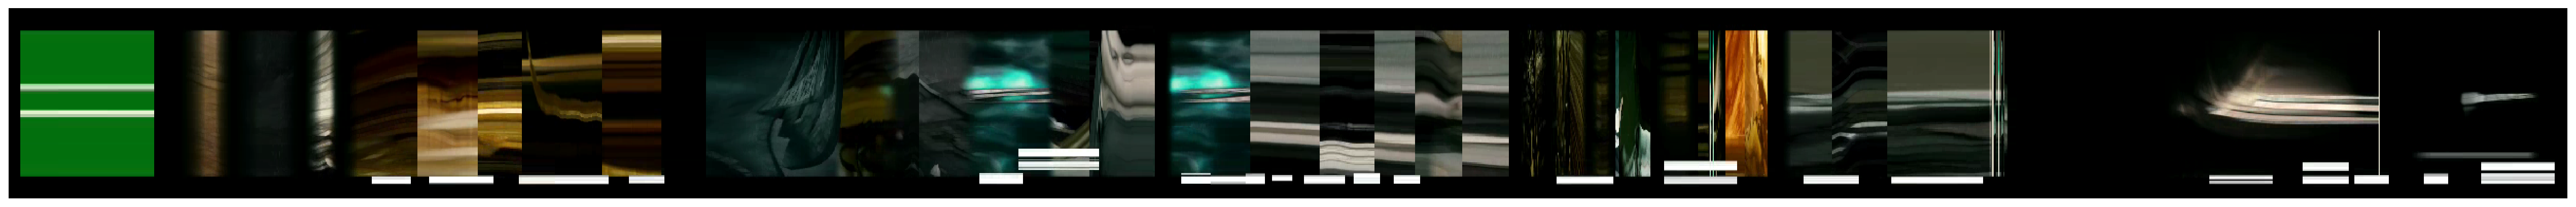
\includegraphics[scale=0.20]{img/harrypotter_1}\label{fig2}}
    \hspace{10mm}
    \subfloat[Aplicacação de Harris]{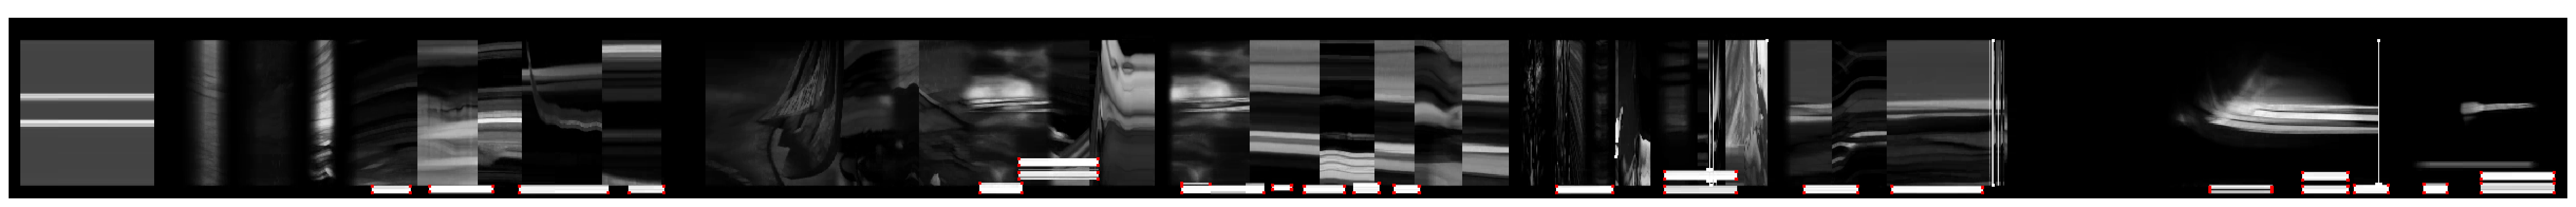
\includegraphics[scale=0.20]{img/harrypotter_1_t7500000000_harris.eps}\label{fig2Diff}}
    \caption{Encontrando legendas - pontos de contornos das legendas
      realçados em vermelho}
  \end{center}
\end{figure}

\newpage
\section{Conclusão}
Pode-se dizer que o detector de contornos de Harris pode 
ser usado para a detecção de padrões de legendas em imagens de ritmo visual a
partir do detector de Harris.
Dependendo do limiar, encontra-se todas as legendas, com um pouco de
pontos fora das curvas das legendas, mas que são indentificáveis e descartáveis.
% Necessária?
% \section{Agradecimentos}

% ******************************************************
% REFERENCIAS BIBLIOGRÁFICAS
% ******************************************************
% \section{Referências}
\bibliographystyle{plain}
\begin{small}
  \bibliography{referencias}
\end{small}

\end{document}
